\chapter{Développement d'un système de plugins entrées/sorties}

\section{Définition de la mission}
\subsection{Contexte}
Dès le début du développement de Vahana VR, la question des entrées et des sorties
du logicel s'était posée. En effet, Studio étant un logiciel de montage de vidéos
360, ses seules entrées sont des fichiers vidéos, issus des caméras de la monture,
comme présenté dans la section \cf{importation-videos}. De même, la sortie proposée 
est l'équirectangulaire représentant la vidéo 360 obtenue, comme présenté dans la section \cf{exportation}.\\
Ce qui est ici appellé \emph{entrées} sont les données envoyées au programme, quand
les \emph{sorties} sont les données émises par ce programme en retour.\\
Et, contrairement à Studio, pour permettre la vidéo 360 en direct, Vahana VR s'affranchit des fichiers
vidéos importés et propose de capturer directement les images des caméras, via
des cartes d'acquisitions branchées sur la machine utilisée. De même, le logiciel peut émettre 
plusieurs fluxs en sortie permettant, par exemple, le \textit{streaming} ou encore la réémissions vers
une carte d'acquisition, l'export d'un equirectangulaire sous forme de fichier
sur le disque dur étant toujours possible.\\
\begin{figure}
  \centering
  \caption{Schéma des entrées/sorties de Vahana VR}
\end{figure}

\subsection{Problématique}
Dès lors, Vahana VR étant destiné à des sociétés de production, le logiciel doit
être compatible avec un maximum de standards, caméras et cartes d'acquisitions vidéos
pour être facilement adopté. Cependant, tout matériel informatique récquérant des pilotes
\footnote{Programme permettant au système d'exploitation d'interagir avec le matériel couvert par ce pilote\cite{pilote-informatique}.}
, et, les besoins des clients en entrées-sorties n'étant pas les mêmes, il n'était
alors pas possible de concevoir un logiciel monolithique contenant tous les programmes 
d'entrées-sorties supportés~: chaque installation du logiciel aurait requis au client 
une installation de l'ensemble des pilotes.\\
De plus, un client pourrait souhaiter utiliser du matériel entrée/sortie encore
non supporté. Il serait intéressant qu'il puisse réaliser son propre développement
dans l'ecosystème de Vahana VR; ainsi le logiciel pourrait devenir virtuellement
compatible avec n'importe quel standard, caméra ou carte d'acquisition.\\
Il fallait donc développer un système assurant à la fois la compatibilité
entre Vahana VR et ces matériels, et intégrant les contraintes exposées.\\

\subsection{Objectifs}
Au début de ce stage, une solution avait déjà été esquissée et était déjà en partie
mise à l'\oe uvre. Cependant un certain travail était encore nécessaire.\\
L'approche retenue de cette solution est celle de la \emph{Programmation Orientée Composant} (POC),
qui permet une certaine modularité dans l'architecture du projet\cite{poc}. Ainsi chaque nouvelle
carte d'acquisition donnera lieu à un nouveau composant, sous forme d'un \textit{plugin},
qui pourra être distribué, chargé et utilisé si nécessaire\cite{plugin}.\\
\newline
Les objectifs retenus pour cette mission ont donc été~:
\begin{itemize}
  \item Développer les entrées HDMI\footnote{\textit{High Definition Multimedia Interface}, 
  norme de diffusion audio/vidéo numérique\cite{hdmi}.} et SDI\footnote{\textit{Serial Digital Interface}, 
  protocole de diffusion vidéo numérique\cite{sdi}.}.
  \item Développer les sorties HDMI et SDI.
  \item Développer des entrées-sorties Ethernet et PCIe\footnote{\textit{PCI Express}, standard
  de connexion de cartes d'extension sur la carte mère d'un ordinateur\cite{pci-express}.}
  spécifiques, à la demande d'un client.
  \item Déployer l'ensemble des \textit{plugins} sur un dépôt séparé.
  \item Documenter et vérifier la bonne intégration des plugins dans Vahana VR.
\end{itemize}

\begin{figure}
  \centering
  \begin{minipage}{0.2\textwidth}
    \centering
    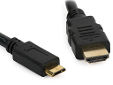
\includegraphics[width=3cm]{images/hdmi-cable.jpg}
    \captionof{subfigure}{HDMI}
  \end{minipage}%
  \hspace{0.03\textwidth}
  \begin{minipage}{0.2\textwidth}
    \centering
    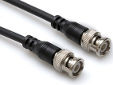
\includegraphics[width=3cm]{images/sdi-cable.jpg}
    \captionof{subfigure}{SDI}
  \end{minipage}%
  \hspace{0.03\textwidth}
  \begin{minipage}{0.2\textwidth}
    \centering
    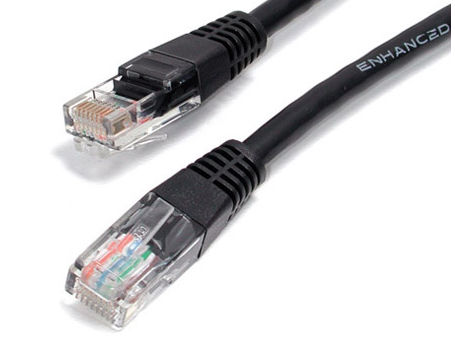
\includegraphics[width=3cm]{images/ethernet-cable.jpg}
    \captionof{subfigure}{Ethernet}
  \end{minipage}%
  \hspace{0.03\textwidth}
  \begin{minipage}{0.2\textwidth}
    \centering
    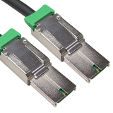
\includegraphics[width=3cm]{images/pcie-cable.jpg}
    \captionof{subfigure}{PCIe}
  \end{minipage}
  \caption{Illustration des différents connecteurs utilisées par Vahana VR}
\end{figure}

\section{Réalisation}
\subsection{Architecture de la solution}


\subsection{Conception type d'un plugin}

\subsection{Quelques difficultés et solutions spécifiques}


\section{Déploiement}
\subsection{Création du dépôt VideoStitch-IO}

\subsection{Documentation}

\subsection{Tests et \textit{QA} de l'intégration des plugins}


\section{Bilan et suite}

